%==============================================================================
%  MATH 231 -- Linear Algebra I (Queens College, Fall 2026)
%  COMPUTATIONAL UNIT, PART 4 -- The Gram-Schmidt Process
%
%  Section numbering runs CONTINUOUSLY across the parts of the computational
%  unit:
%
%      Part 1  MATH231_computational_1_operation_counting        Sections 1-4
%      Part 2  MATH231_computational_2_k_nearest_neighbours      Sections 5-10
%      Part 3  MATH231_computational_3_k_means_clustering        Sections 11-15
%      Part 4  MATH231_computational_4_gram_schmidt              Sections 16-20
%
%  Hence \setcounter{section}{15}: this part opens at Section 16.
%
%  STATUS: complete.  Sections 16-20.
%
%  AUDIENCE: distributed to students.  No instructor-facing apparatus.
%
%  THIS PART COLLECTS A DEBT.  The vector unit closes Sec. 21.6 with a
%  Looking-ahead that names Gram-Schmidt outright and describes its mechanism
%  ("subtract off the projection, as in Sec. 12.6, so that what remains is
%  orthogonal to what came before").  Sec. 16 opens by pointing at that promise.
%  Do not re-derive Sec. 21.6's orthogonal-basis coordinate formula from
%  scratch -- Sec. 16.4 cites it and shows normalisation kills the denominator.
%
%  CORRECTIONS against the drafted outline.
%
%   1. PROJECTION SUBSCRIPT.  The outline wrote "w = u - proj_u(v)" and then
%      "w is orthogonal to u".  Under the convention fixed in the vector unit
%      (Sec. 12.4: "the subscript names the vector you are projecting ONTO"),
%      proj_u(v) is the shadow of v ON u, so u - proj_u(v) is a multiple of u,
%      not something orthogonal to it.  The form the vector unit actually
%      establishes -- Sec. 12.6, and drawn there -- is
%
%          v - proj_u(v)  is orthogonal to  u.
%
%      That is what is used here.  It also matches the outline's own next two
%      claims ("w is orthogonal to u"; "we have 2 vectors that are orthogonal,
%      namely w and u"), so only the normalisation line needed adjusting: the
%      pair to normalise is {u, w}, giving u-hat and w-hat, not v-hat.
%
%   2. delta COLLISION.  Part 2 uses delta_i for the distance from the query to
%      x_i (Sec. 7.4, Sec. 8.3).  The Kronecker delta introduced in Sec. 16.2 is
%      a different object wearing the same letter, inside the same unit.  A
%      "common confusion" box in 16.2 names the clash rather than hoping nobody
%      notices.
%
%  CLASSICAL vs MODIFIED.  Line 4 of the pseudocode dots against the ORIGINAL
%  v_k, which is classical Gram-Schmidt.  Modified Gram-Schmidt dots against the
%  running w instead -- algebraically identical, numerically not.  Sec. 20.3
%  flags the distinction and defers it, since the outline says the algorithm
%  will be revisited.  Do not silently write the modified form here; the whole
%  point of the later treatment is that the two differ.
%
%  THE WORKED EXAMPLE (Sec. 18.3) is v1=[1,1,0], v2=[1,0,1], v3=[0,1,1], chosen
%  because every q comes out with a clean radical: q1 = [1,1,0]/sqrt2,
%  q2 = [1,-1,2]/sqrt6, q3 = [-1,1,1]/sqrt3.  Sec. 18.4 then reads the
%  coordinates of u = [1,2,3] against that basis and verifies the reconstruction
%  exactly -- that check is the payoff of Sec. 16 and should not be cut.
%
%  Compile with pdflatex (standard TeX Live packages only; uses tikz).
%==============================================================================
\documentclass[11pt]{article}

\usepackage[margin=1in]{geometry}
\usepackage{amsmath,amssymb,amsthm}
\usepackage[dvipsnames]{xcolor}
\usepackage{enumitem}
\usepackage{booktabs}
\usepackage{array}
\usepackage[hidelinks]{hyperref}
\usepackage{titlesec}
\usepackage{needspace}
\usepackage{tikz}
\usetikzlibrary{arrows.meta,shapes.geometric}

%------------------------------------------------------------------ style ----
\titleformat{\section}{\large\bfseries\sffamily}{\thesection.}{0.6em}{}
\titleformat{\subsection}{\normalsize\bfseries\sffamily}{\thesubsection.}{0.5em}{}
\titlespacing*{\section}{0pt}{14pt}{6pt}

\theoremstyle{plain}
\newtheorem{thm}{Theorem}[section]
\newtheorem{lem}[thm]{Lemma}

\theoremstyle{definition}
\newtheorem{defn}{Definition}[section]
\newtheorem{ex}{Example}[section]
\theoremstyle{remark}
\newtheorem*{rmk}{Remark}
\newtheorem*{warn}{A common confusion}

\newcommand{\lookahead}{\par\smallskip\noindent
  \textbf{\sffamily\textcolor{RoyalBlue}{Looking ahead.}}\ \ignorespaces}
\newcommand{\lookback}{\par\smallskip\noindent
  \textbf{\sffamily\textcolor{ForestGreen}{From the vector unit.}}\ \ignorespaces}

%--------------------------------------------------------------- notation ----
\newcommand{\R}{\mathbb{R}}
\newcommand{\vc}[1]{\mathbf{#1}}
\newcommand{\norm}[1]{\lVert #1\rVert}
\newcommand{\ip}[2]{\langle #1,\, #2\rangle}
\newcommand{\proj}[2]{\operatorname{proj}_{#1}(#2)}
\newcommand{\uv}[1]{\hat{\vc{#1}}}
\newcommand{\spn}{\operatorname{span}}

%--------------------------------------------------------------- pseudocode --
\newcommand{\kw}[1]{\textsf{\bfseries #1}}
\newcommand{\ind}{\hspace*{1.3em}}
\newcommand{\indd}{\hspace*{2.6em}}
\newcounter{algoline}
\newenvironment{algo}[2]{%
  \par\medskip\needspace{8\baselineskip}%
  \begin{center}\begin{minipage}{0.94\textwidth}%
  \hrule height 0.9pt \vspace{3pt}%
  \noindent{\sffamily\bfseries #1}\par\vspace{2pt}%
  \noindent{\small #2}\par\vspace{3pt}%
  \hrule height 0.4pt \vspace{5pt}%
  \begin{list}{\textbf{\arabic{algoline}:}}%
    {\usecounter{algoline}\setlength{\leftmargin}{2.3em}%
     \setlength{\labelwidth}{1.8em}\setlength{\labelsep}{0.5em}%
     \setlength{\itemsep}{2pt}\setlength{\topsep}{0pt}%
     \setlength{\parsep}{0pt}}%
}{%
  \end{list}\vspace{5pt}\hrule height 0.9pt%
  \end{minipage}\end{center}\medskip%
}

%------------------------------------------------------------- tikz helpers --
\tikzset{
  vecarr/.style   = {-{Stealth[length=2.6mm,width=2.0mm]}, thick},
  axisline/.style = {->, gray!75, thin},
  plane/.style    = {draw=gray!55, fill=gray!12}
}

\title{\vspace{-1.2cm}\textbf{\sffamily MATH 231 -- Linear Algebra I}\\[4pt]
       {\large\sffamily The Computational Unit, Part 4 \textbullet\
        The Gram--Schmidt Process}\\[2pt]
       {\normalsize\sffamily Kiely Hall 326 \textbullet\
        Instructor: Kevin Bedoya}}
\author{}
\date{}

\begin{document}
\setcounter{section}{15}  % this part opens at Section 16; see the header note
\maketitle
\vspace{-1.6cm}

\noindent\textbf{About this document.} The vector unit ended one of its sections
with a promise. It had just shown that against an \emph{orthogonal} basis,
coordinates cost nothing to find, and then asked whether such a basis can always
be manufactured out of an ordinary one. It said yes, named the procedure, and
stopped. This part is that procedure.

\begin{center}
\renewcommand{\arraystretch}{1.2}
\begin{tabular}{@{}l l l@{}}
\toprule
\textbf{Part} & \textbf{Sections} & \textbf{Subject} \\
\midrule
1 & \S1--\S4    & operation counting, Big-O, floating point, error \\
2 & \S5--\S10   & $k$-nearest neighbours \\
3 & \S11--\S15  & $k$-means clustering \\
4 & \S16--\S20  & the Gram--Schmidt process \\
\bottomrule
\end{tabular}
\end{center}

\begin{warn}[Whose \S16 is this?]
Section numbering runs continuously through the computational unit, so a bare
``\S18.2'' below means \S18.2 \emph{of this unit}. References into the vector
unit or the matrix unit always name them.
\end{warn}

\medskip
\noindent\textbf{Assumed.} This part expects the whole vector unit and the first
part of the matrix unit. Specifically --- from the vector unit: span, linear
independence, basis and dimension (\S17--\S19); the dot product and its
bilinearity (\S11.8, \S21.1); the norm, unit vectors and normalisation
(\S11.9); projection and the orthogonal piece $\vc{v}-\proj{\vc{u}}{\vc{v}}$
(\S12.4, \S12.6); orthogonality, orthonormality, and why an orthogonal basis is
worth having (\S16, \S21.6); $\R^{n}$ and $n$-dimensional notation (\S24). From
the matrix unit: the coordinate problem written as a linear system (\S1), and
the same system compressed to the matrix--vector product $\mathsf{V}\vc{x}=\vc{u}$
(\S2.4). From this unit: Big-O (\S2.7) and FLOP counting (\S4.6).

\medskip
\noindent\textbf{What you should be able to do afterwards.} State what an
orthonormal set is and write it with the Kronecker delta; explain why
coordinates against an orthonormal basis are dot products and no system need be
solved; carry out Gram--Schmidt by hand in $\R^{2}$ and $\R^{3}$; write its
pseudocode; say exactly what happens when the input vectors are dependent, in
exact arithmetic and in floating point; and count the algorithm's operations and
give its complexity.

%==============================================================================
\section{Reading coordinates without solving}
%==============================================================================

%------------------------------------------------------------------------------
\subsection{What the basis left us with}
%------------------------------------------------------------------------------
Take $n$ linearly independent vectors $\vc{v}_{1},\dots,\vc{v}_{n}$ in
$\R^{n}$. Being independent and $n$ of them, they span $\R^{n}$: every vector in
the space is reachable as a linear combination of them, and --- this is the part
that matters --- reachable in exactly one way. So for any $\vc{u}\in\R^{n}$
there are unique numbers $\alpha_{1},\dots,\alpha_{n}$ with
\begin{equation}\label{eq:general}
  \vc{u} \;=\; \alpha_{1}\vc{v}_{1} + \alpha_{2}\vc{v}_{2}
           + \cdots + \alpha_{n}\vc{v}_{n} .
\end{equation}
Those $\alpha$'s are the \emph{coordinates} of $\vc{u}$ against that basis. The
basis guarantees they exist. It does not tell you what they are.

\lookback The matrix unit took up exactly this question. Writing
\eqref{eq:general} out one component at a time produces $n$ simultaneous linear
equations in the $n$ unknowns $\alpha_{1},\dots,\alpha_{n}$ (matrix unit \S1),
and stacking the $\vc{v}_{j}$ as the columns of a matrix compresses all $n$
equations into the single statement $\mathsf{V}\vc{x}=\vc{u}$ (matrix unit
\S2.4). What neither section did was \emph{solve} it.

That is the state we are in. We can pose the problem and we can write it
compactly, and for $n=2$ we can grind it out by hand. But nothing about the
compact notation makes the work smaller. There are still $n$ unknowns
constrained by $n$ equations that must all hold at once, and no equation can be
settled in isolation --- change one $\alpha$ and every component of the sum
moves. For $n=2$ that is a nuisance. For $n=500$, which is a small number of
features by the standards of \S5.1, it is a serious computation.

So the honest summary is: a basis promises the coordinates are there, and then
hands you a system of equations.

Unless we choose the basis more carefully.

%------------------------------------------------------------------------------
\subsection{Orthonormal vectors, and the Kronecker delta}
%------------------------------------------------------------------------------
\lookback A set of vectors is \textbf{orthonormal} when the vectors are
mutually orthogonal and each has length one (vector unit \S16). For two of them,
$\vc{q}_{i}$ and $\vc{q}_{j}$, that is two statements:
\[
  \ip{\vc{q}_{i}}{\vc{q}_{j}} = 0 \ \ (i\neq j),
  \qquad\qquad
  \ip{\vc{q}_{i}}{\vc{q}_{i}} = 1 .
\]
The first is orthogonality; the second is unit length, since
$\ip{\vc{q}}{\vc{q}}=\norm{\vc{q}}^{2}$ and $\norm{\vc{q}}=1$.

Those two conditions get written together often enough that they have a
shorthand.

\begin{defn}[Kronecker delta]
The \textbf{Kronecker delta} $\delta_{ij}$ is the function
\[
  \delta_{ij} \;=\;
  \begin{cases}
    1 & \text{if } i = j,\\[2pt]
    0 & \text{if } i \neq j .
  \end{cases}
\]
\end{defn}

\noindent With it, the whole of orthonormality is one equation:
\begin{equation}\label{eq:orthonormal}
  \ip{\vc{q}_{i}}{\vc{q}_{j}} \;=\; \delta_{ij} .
\end{equation}

The delta is not deep --- it is a lookup table with two entries. What makes it
worth a name is what it does inside a sum. Every term of
$\sum_{j}\beta_{j}\delta_{ji}$ is zero except the one where $j=i$, which
survives with $\delta_{ii}=1$:
\begin{equation}\label{eq:sift}
  \sum_{j=1}^{n} \beta_{j}\,\delta_{ji} \;=\; \beta_{i} .
\end{equation}
A sum of $n$ terms collapses to one. Read $\delta$ as an instruction: \emph{keep
the matching index, delete everything else}.

\begin{warn}[Two different $\delta$'s in this unit]
Part 2 used $\delta_{i}$ for the distance from the query point to $\vc{x}_{i}$
(\S7.4, \S8.3). That is an unrelated object that happens to wear the same
letter. Tell them apart by the indices: the Kronecker delta always carries
\emph{two}, and it is only ever $0$ or $1$.
\end{warn}

%------------------------------------------------------------------------------
\subsection{The coordinates fall out}
%------------------------------------------------------------------------------
Now suppose the $n$ vectors we were handed are not merely independent but
orthonormal. Call them $\vc{q}_{1},\dots,\vc{q}_{n}$. They are still $n$
independent vectors in $\R^{n}$ --- orthogonal vectors are independent, which is
the vector unit's \S21.2 --- so they still span, and \eqref{eq:general} still
applies. Write it with new letters for the coordinates:
\begin{equation}\label{eq:onb}
  \vc{u} \;=\; \beta_{1}\vc{q}_{1} + \beta_{2}\vc{q}_{2}
           + \cdots + \beta_{n}\vc{q}_{n} .
\end{equation}
Everything so far is identical to \S16.1. Here is where it stops being
identical: take the dot product of both sides with $\vc{q}_{1}$.

The dot product is bilinear (vector unit \S21.1), so it distributes across the
sum and pulls the scalars out:
\[
  \ip{\vc{u}}{\vc{q}_{1}}
  \;=\; \beta_{1}\underbrace{\ip{\vc{q}_{1}}{\vc{q}_{1}}}_{=\,1}
      + \beta_{2}\underbrace{\ip{\vc{q}_{2}}{\vc{q}_{1}}}_{=\,0}
      + \cdots
      + \beta_{n}\underbrace{\ip{\vc{q}_{n}}{\vc{q}_{1}}}_{=\,0}
  \;=\; \beta_{1} .
\]
Every term but the first vanishes. Not because of anything about $\vc{u}$, and
not because of any cleverness --- they vanish because the basis was built so
that they would.

Nothing distinguished $\vc{q}_{1}$, so dot with $\vc{q}_{i}$ instead and the
same collapse happens around the $i$-th term. In the delta notation it is one
line, using \eqref{eq:orthonormal} and then the sifting property
\eqref{eq:sift}:
\[
  \ip{\vc{u}}{\vc{q}_{i}}
  \;=\; \Bigl\langle \sum_{j=1}^{n}\beta_{j}\vc{q}_{j},\ \vc{q}_{i}\Bigr\rangle
  \;=\; \sum_{j=1}^{n}\beta_{j}\ip{\vc{q}_{j}}{\vc{q}_{i}}
  \;=\; \sum_{j=1}^{n}\beta_{j}\delta_{ji}
  \;=\; \beta_{i} .
\]

\begin{thm}[Coordinates against an orthonormal basis]\label{thm:coords}
Let $\{\vc{q}_{1},\dots,\vc{q}_{n}\}$ be an orthonormal basis of $\R^{n}$ and
let $\vc{u}\in\R^{n}$. Then the coordinates of $\vc{u}$ are its dot products
with the basis vectors:
\[
  \beta_{i} \;=\; \ip{\vc{u}}{\vc{q}_{i}},
  \qquad\text{so}\qquad
  \vc{u} \;=\; \ip{\vc{u}}{\vc{q}_{1}}\vc{q}_{1}
             + \ip{\vc{u}}{\vc{q}_{2}}\vc{q}_{2}
             + \cdots
             + \ip{\vc{u}}{\vc{q}_{n}}\vc{q}_{n} .
\]
\end{thm}

No system was solved. The coordinates were \emph{read off}.

%------------------------------------------------------------------------------
\subsection{What that saved}
%------------------------------------------------------------------------------
It is worth being precise about the size of the win, because it is not a small
constant factor.

Against a general basis, the $n$ coordinates are entangled: they are the
solution of a coupled system, and you cannot know any one of them until you have
essentially done the work for all of them. Against an orthonormal basis they are
\emph{independent of each other}. Coordinate $\beta_{7}$ is one dot product. You
can compute it without ever looking at $\beta_{3}$, compute the coordinates in
any order, compute only the ones you want, or compute them on separate machines
at the same time.

\lookback The vector unit reached this conclusion for an orthogonal basis in
\S21.6, where the coordinate came out as
\[
  \alpha \;=\; \frac{\ip{\vc{u}}{\vc{w}}}{\norm{\vc{u}}^{2}} .
\]
Orthonormality is that formula with the denominator deleted. Normalising each
basis vector makes $\norm{\vc{q}_{i}}^{2}=1$, and the division disappears --- so
an orthonormal basis is an orthogonal basis with the last bit of arithmetic
already paid for. That section also observed that $\vc{u}$ is then the sum of
its own shadows on the basis directions; Theorem~\ref{thm:coords} is that
statement with unit-length shadows, since for $\norm{\vc{q}}=1$ the projection
$\proj{\vc{q}}{\vc{u}}$ is exactly $\ip{\vc{u}}{\vc{q}}\vc{q}$.

\begin{rmk}
Any basis will answer the question. A general basis
$\{\vc{v}_{1},\dots,\vc{v}_{n}\}$ determines $\vc{u}$ just as completely as an
orthonormal one, and \eqref{eq:general} is not wrong. The two differ in what it
costs to \emph{use} them. If the goal is to stitch together a set of directions
that walk you to an arbitrary $\vc{u}$, and to do it repeatedly, an orthonormal
basis is the one to want: same information, no system.
\end{rmk}

This is only useful if we can get such a basis. Bases do not arrive orthonormal.
Where would one even start?

%==============================================================================
\section{Building the basis: one move}
%==============================================================================

%------------------------------------------------------------------------------
\subsection{The move, recalled from \texorpdfstring{$\R^{2}$}{R2}}
%------------------------------------------------------------------------------
We already have the whole idea. It was built in the vector unit for two
dimensions and never called an algorithm.

\lookback Given $\vc{u}\neq\vc{0}$ and any $\vc{v}$, the projection
$\proj{\vc{u}}{\vc{v}}$ is the part of $\vc{v}$ that points along $\vc{u}$,
taken as a vector (\S12.4; the subscript names the vector being projected
\emph{onto}). Subtracting it leaves
\begin{equation}\label{eq:orthpiece}
  \vc{w} \;=\; \vc{v} - \proj{\vc{u}}{\vc{v}} ,
\end{equation}
and \S12.6 showed that $\vc{w}\perp\vc{u}$. The reason is geometric rather than
computational: $\proj{\vc{u}}{\vc{v}}$ is precisely the amount of $\vc{v}$ that
lies along $\vc{u}$, so once it is removed, what is left has no component in the
$\vc{u}$ direction at all. Nothing is left to be orthogonal about.

Confirm it in one line. Using bilinearity and
$\proj{\vc{u}}{\vc{v}}=\bigl(\ip{\vc{u}}{\vc{v}}/\norm{\vc{u}}^{2}\bigr)\vc{u}$,
\[
  \ip{\vc{w}}{\vc{u}}
  = \ip{\vc{v}}{\vc{u}} - \frac{\ip{\vc{u}}{\vc{v}}}{\norm{\vc{u}}^{2}}
    \ip{\vc{u}}{\vc{u}}
  = \ip{\vc{v}}{\vc{u}} - \ip{\vc{u}}{\vc{v}}
  = 0 .
\]
The subtraction is engineered to make this cancellation happen; the coefficient
on $\vc{u}$ is chosen for no other purpose.

%------------------------------------------------------------------------------
\subsection{Two dimensions, finished}
%------------------------------------------------------------------------------
In $\R^{2}$ that single move has already done most of the job. Start with any
basis $\{\vc{u},\vc{v}\}$ --- independent, otherwise arbitrary. Set
$\vc{w}=\vc{v}-\proj{\vc{u}}{\vc{v}}$. Then $\vc{u}\perp\vc{w}$, and we have
two orthogonal vectors where we had two skew ones.

That is an orthogonal basis, not yet an orthonormal one: the lengths are still
whatever they happened to be. Fix that by normalising each, which the vector
unit's \S11.9 does by dividing a vector by its own length:
\[
  \uv{q}_{1} = \frac{\vc{u}}{\norm{\vc{u}}},
  \qquad
  \uv{q}_{2} = \frac{\vc{w}}{\norm{\vc{w}}} .
\]
Both now have length one, and scaling a vector does not change its direction, so
they are still orthogonal. Two orthonormal vectors in $\R^{2}$, built out of an
arbitrary basis, by one subtraction and two divisions.

\begin{center}
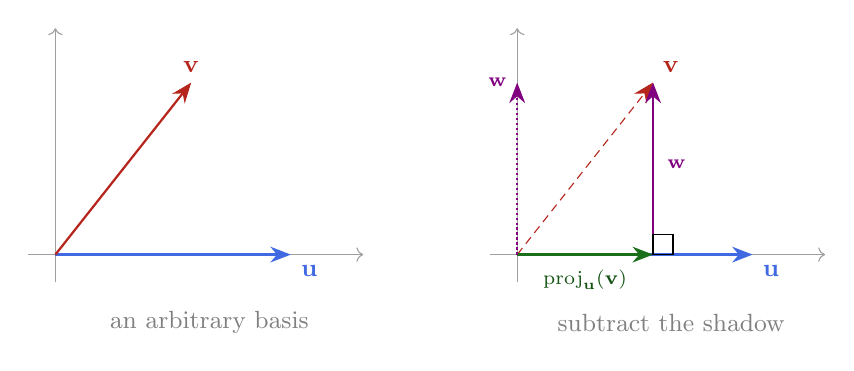
\begin{tikzpicture}[scale=1.15]
  % --- left: before
  \begin{scope}
    \draw[axisline] (-0.3,0) -- (3.4,0);
    \draw[axisline] (0,-0.3) -- (0,2.5);
    \draw[vecarr,RoyalBlue] (0,0) -- (2.6,0) node[below right,font=\small]{$\vc{u}$};
    \draw[vecarr,BrickRed]  (0,0) -- (1.5,1.9) node[above,font=\small]{$\vc{v}$};
    \node[font=\small,gray] at (1.7,-0.75) {an arbitrary basis};
  \end{scope}
  % --- right: after
  \begin{scope}[xshift=5.1cm]
    \draw[axisline] (-0.3,0) -- (3.4,0);
    \draw[axisline] (0,-0.3) -- (0,2.5);
    \draw[vecarr,RoyalBlue] (0,0) -- (2.6,0) node[below right,font=\small]{$\vc{u}$};
    \draw[vecarr,BrickRed,densely dashed,thin]  (0,0) -- (1.5,1.9)
          node[above right,font=\small]{$\vc{v}$};
    % projection along u
    \draw[vecarr,ForestGreen!80!black] (0,0) -- (1.5,0);
    \node[below,font=\scriptsize,ForestGreen!60!black] at (0.75,-0.06)
         {$\proj{\vc{u}}{\vc{v}}$};
    % w = v - proj, drawn from the head of proj to the head of v
    \draw[vecarr,Purple] (1.5,0) -- (1.5,1.9);
    \node[right,font=\scriptsize,Purple] at (1.55,1.0) {$\vc{w}$};
    % w moved to the origin
    \draw[vecarr,Purple,densely dotted] (0,0) -- (0,1.9)
          node[left,font=\scriptsize]{$\vc{w}$};
    \draw (1.5,0) rectangle (1.72,0.22);
    \node[font=\small,gray] at (1.7,-0.75) {subtract the shadow};
  \end{scope}
\end{tikzpicture}
\end{center}

\noindent The right-hand picture is the entire algorithm in miniature. Everything
that follows is this move, applied again.

%------------------------------------------------------------------------------
\subsection{Three dimensions}
%------------------------------------------------------------------------------
Now take three independent vectors $\vc{v}_{1},\vc{v}_{2},\vc{v}_{3}$ in
$\R^{3}$ and do it again, one vector at a time. The rule is the same at every
step: \emph{strip off everything that points along the directions already
fixed}.

\medskip
\noindent\textbf{Step 1.} There is nothing to be orthogonal to yet, so the first
direction is free. Keep $\vc{v}_{1}$ and give it unit length:
\[
  \vc{w}_{1} = \vc{v}_{1},
  \qquad
  \vc{q}_{1} = \frac{\vc{w}_{1}}{\norm{\vc{w}_{1}}} .
\]

\medskip
\noindent\textbf{Step 2.} Take $\vc{v}_{2}$ and remove its $\vc{q}_{1}$
component. Because $\vc{q}_{1}$ is already a unit vector, its projection
coefficient needs no denominator --- $\proj{\vc{q}_{1}}{\vc{v}_{2}}
= \ip{\vc{v}_{2}}{\vc{q}_{1}}\vc{q}_{1}$:
\[
  \vc{w}_{2} = \vc{v}_{2} - \ip{\vc{v}_{2}}{\vc{q}_{1}}\vc{q}_{1},
  \qquad
  \vc{q}_{2} = \frac{\vc{w}_{2}}{\norm{\vc{w}_{2}}} .
\]
This is \S17.2 verbatim. Now $\vc{q}_{1}\perp\vc{q}_{2}$, both unit length, and
together they span a \emph{plane} through the origin --- a two-dimensional
subspace of $\R^{3}$, in the sense of the vector unit's \S22.2.

\medskip
\noindent\textbf{Step 3.} Here is the one genuinely new step, and the reason
three dimensions is worth drawing. $\vc{v}_{3}$ sticks out of that plane. It has
a component along $\vc{q}_{1}$ and a component along $\vc{q}_{2}$, and both must
go:
\[
  \vc{w}_{3} = \vc{v}_{3}
             - \ip{\vc{v}_{3}}{\vc{q}_{1}}\vc{q}_{1}
             - \ip{\vc{v}_{3}}{\vc{q}_{2}}\vc{q}_{2},
  \qquad
  \vc{q}_{3} = \frac{\vc{w}_{3}}{\norm{\vc{w}_{3}}} .
\]
The two subtracted terms are together the \emph{shadow of $\vc{v}_{3}$ on the
plane}: they are exactly the coordinates Theorem~\ref{thm:coords} would read off
if $\vc{v}_{3}$ lay in that plane. Removing them leaves the part of $\vc{v}_{3}$
that the plane cannot see --- the vertical drop from the tip of $\vc{v}_{3}$
straight down to the plane.

\Needspace*{16\baselineskip}
\begin{center}
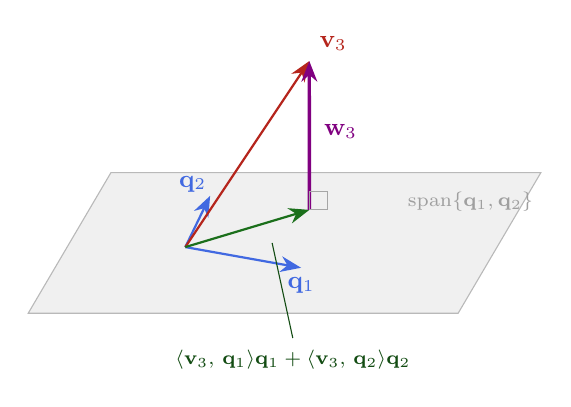
\begin{tikzpicture}[scale=1.05]
  % the plane spanned by q1,q2
  \fill[plane] (-0.9,-0.75) -- (4.3,-0.75) -- (5.3,0.95) -- (0.1,0.95) -- cycle;
  \node[font=\scriptsize,gray!75] at (4.45,0.60) {$\spn\{\vc{q}_{1},\vc{q}_{2}\}$};
  \coordinate (O) at (1.0,0.05);
  \coordinate (P) at (2.5,0.5);
  % in-plane orthonormal pair, aimed apart so no label crowds the shadow
  \draw[vecarr,RoyalBlue] (O) -- (2.40,-0.20)
        node[below,font=\small,inner sep=3pt]{$\vc{q}_{1}$};
  \draw[vecarr,RoyalBlue] (O) -- (1.30,0.67)
        node[above left,font=\small,inner sep=1pt]{$\vc{q}_{2}$};
  % v3 out of the plane
  \draw[vecarr,BrickRed] (O) -- (2.5,2.3)
        node[above right,font=\small]{$\vc{v}_{3}$};
  % its shadow on the plane
  \draw[vecarr,ForestGreen!80!black] (O) -- (P);
  \draw[ForestGreen!55!black,thin] (2.05,0.10) -- (2.30,-1.05);
  \node[font=\scriptsize,ForestGreen!55!black,below] at (2.30,-1.08)
       {$\ip{\vc{v}_{3}}{\vc{q}_{1}}\vc{q}_{1}
         +\ip{\vc{v}_{3}}{\vc{q}_{2}}\vc{q}_{2}$};
  % w3: the vertical drop
  \draw[vecarr,Purple,very thick] (P) -- (2.5,2.3);
  \node[right,font=\small,Purple] at (2.56,1.45) {$\vc{w}_{3}$};
  \draw[gray!70] (2.5,0.5) rectangle (2.72,0.72);
\end{tikzpicture}
\end{center}

\noindent Read the picture as a triangle: $\vc{v}_{3}$ is the hypotenuse from
the origin, the green vector is its shadow lying flat in the plane, and
$\vc{w}_{3}$ is the leg joining the shadow's tip to $\vc{v}_{3}$'s tip. That leg
meets the plane at a right angle, so it is orthogonal to \emph{everything} in
the plane --- to $\vc{q}_{1}$, to $\vc{q}_{2}$, and to every combination of
them. Normalising it gives $\vc{q}_{3}$, and
$\{\vc{q}_{1},\vc{q}_{2},\vc{q}_{3}\}$ is an orthonormal basis of $\R^{3}$.

\begin{rmk}
Notice what step 3 did \emph{not} require: it did not go back and adjust
$\vc{q}_{1}$ or $\vc{q}_{2}$. Once a direction is fixed it is never revisited.
Each new vector is cleaned against the directions already built, and then it
joins them. That is what makes the procedure a loop rather than a system.
\end{rmk}

%==============================================================================
\section{The Gram--Schmidt process}
%==============================================================================
The procedure just carried out in $\R^{2}$ and $\R^{3}$ is the
\textbf{Gram--Schmidt process}. It takes a list of linearly independent vectors
and returns an orthonormal list spanning the same space.

%------------------------------------------------------------------------------
\subsection{The general step}
%------------------------------------------------------------------------------
Suppose $\vc{v}_{1},\dots,\vc{v}_{n}$ are linearly independent in $\R^{n}$, and
suppose $\vc{q}_{1},\dots,\vc{q}_{k-1}$ have already been produced. To produce
$\vc{q}_{k}$, subtract from $\vc{v}_{k}$ its component along every direction
built so far, then normalise what is left:
\begin{equation}\label{eq:gs}
  \vc{w}_{k} \;=\; \vc{v}_{k}
    - \sum_{j=1}^{k-1}\ip{\vc{v}_{k}}{\vc{q}_{j}}\,\vc{q}_{j},
  \qquad\qquad
  \vc{q}_{k} \;=\; \frac{\vc{w}_{k}}{\norm{\vc{w}_{k}}} .
\end{equation}
For $k=1$ the sum is empty, so $\vc{w}_{1}=\vc{v}_{1}$ and the first step is
just a normalisation --- consistent with $\S17.3$, where the first direction was
free.

That $\vc{w}_{k}$ really is orthogonal to each earlier $\vc{q}_{i}$ is the
computation of \S17.1 done $k-1$ times at once. Dot \eqref{eq:gs} with
$\vc{q}_{i}$ for some $i<k$, and use bilinearity together with
$\ip{\vc{q}_{j}}{\vc{q}_{i}}=\delta_{ji}$:
\[
  \ip{\vc{w}_{k}}{\vc{q}_{i}}
  = \ip{\vc{v}_{k}}{\vc{q}_{i}}
    - \sum_{j=1}^{k-1}\ip{\vc{v}_{k}}{\vc{q}_{j}}\,\delta_{ji}
  = \ip{\vc{v}_{k}}{\vc{q}_{i}} - \ip{\vc{v}_{k}}{\vc{q}_{i}}
  = 0 .
\]
The delta collapses the sum to its $j=i$ term, which is precisely the quantity
that was subtracted. Every earlier direction is cancelled, and only those.

\begin{rmk}[The spans match at every stage]
Gram--Schmidt does not merely produce \emph{some} orthonormal basis --- it
produces one aligned with the input list, in the sense that
\[
  \spn\{\vc{q}_{1},\dots,\vc{q}_{k}\}
  \;=\;
  \spn\{\vc{v}_{1},\dots,\vc{v}_{k}\}
  \qquad\text{for every } k .
\]
Each $\vc{q}_{k}$ is built only out of $\vc{v}_{k}$ and earlier $\vc{q}$'s, so
it adds nothing new to the span; and $\vc{v}_{k}$ can be recovered from
$\vc{q}_{1},\dots,\vc{q}_{k}$ by undoing \eqref{eq:gs}. The two lists sweep out
the same nested sequence of subspaces --- the same line, then the same plane,
then the same three-dimensional space, and so on.
\end{rmk}

%------------------------------------------------------------------------------
\subsection{Pseudocode}
%------------------------------------------------------------------------------
\begin{algo}{Gram--Schmidt}{%
  \textbf{Input:} linearly independent $\vc{v}_{1},\dots,\vc{v}_{n}\in\R^{n}$.\quad
  \textbf{Output:} orthonormal $\vc{q}_{1},\dots,\vc{q}_{n}$ with
  $\spn\{\vc{q}_{1},\dots,\vc{q}_{k}\}=\spn\{\vc{v}_{1},\dots,\vc{v}_{k}\}$ for
  all $k$.}
\item \kw{for} $k = 1,\dots,n$:
\item \ind $\vc{w} \;\gets\; \vc{v}_{k}$
        \hfill\textit{\small start from the raw vector}
\item \ind \kw{for} $j = 1,\dots,k-1$:
\item \indd $\vc{w} \;\gets\; \vc{w} - \ip{\vc{v}_{k}}{\vc{q}_{j}}\,\vc{q}_{j}$
        \hfill\textit{\small strip the $\vc{q}_{j}$ component}
\item \ind $\vc{q}_{k} \;\gets\; \vc{w}\,/\,\norm{\vc{w}}$
        \hfill\textit{\small normalise what survives}
\item \kw{return} $\vc{q}_{1},\dots,\vc{q}_{n}$
\end{algo}

\noindent Two lines deserve a second look.

\textbf{Line 4} dots against $\vc{v}_{k}$, the \emph{original} vector, not
against the partially-stripped $\vc{w}$. In exact arithmetic it makes no
difference which you use: $\vc{w}$ differs from $\vc{v}_{k}$ only by multiples
of $\vc{q}_{1},\dots,\vc{q}_{j-1}$, all of which are orthogonal to $\vc{q}_{j}$
and so contribute nothing to the dot product. In floating-point arithmetic it
makes a substantial difference. We return to this in \S20.3.

\textbf{Line 5} divides by $\norm{\vc{w}}$, and divides without checking it. That
is safe exactly when the inputs are independent, which is why the input line
says so. \S19 is about what happens when they are not.

%------------------------------------------------------------------------------
\subsection{A worked example}
%------------------------------------------------------------------------------
\begin{ex}
Orthonormalise
\[
  \vc{v}_{1}=[\,1,\,1,\,0\,],\qquad
  \vc{v}_{2}=[\,1,\,0,\,1\,],\qquad
  \vc{v}_{3}=[\,0,\,1,\,1\,] .
\]

\smallskip
\noindent\textbf{$k=1$.} Nothing to subtract. $\norm{\vc{v}_{1}}=\sqrt{2}$, so
\[
  \vc{q}_{1}=\tfrac{1}{\sqrt{2}}[\,1,\,1,\,0\,] .
\]

\smallskip
\noindent\textbf{$k=2$.}
$\ip{\vc{v}_{2}}{\vc{q}_{1}}=\tfrac{1}{\sqrt2}(1\cdot1+0\cdot1+1\cdot0)
=\tfrac{1}{\sqrt2}$, so
\[
  \vc{w}_{2}=[\,1,\,0,\,1\,]-\tfrac{1}{\sqrt2}\cdot\tfrac{1}{\sqrt2}[\,1,\,1,\,0\,]
            =[\,1,\,0,\,1\,]-\tfrac12[\,1,\,1,\,0\,]
            =\bigl[\,\tfrac12,\,-\tfrac12,\,1\,\bigr] .
\]
Then $\norm{\vc{w}_{2}}^{2}=\tfrac14+\tfrac14+1=\tfrac32$, and clearing the
fraction by factoring out $\tfrac12$,
\[
  \vc{q}_{2}=\frac{\tfrac12[\,1,\,-1,\,2\,]}{\sqrt{3/2}}
            =\tfrac{1}{\sqrt{6}}[\,1,\,-1,\,2\,] .
\]

\smallskip
\noindent\textbf{$k=3$.} Two components to remove:
\[
  \ip{\vc{v}_{3}}{\vc{q}_{1}}=\tfrac{1}{\sqrt2}(0+1+0)=\tfrac{1}{\sqrt2},
  \qquad
  \ip{\vc{v}_{3}}{\vc{q}_{2}}=\tfrac{1}{\sqrt6}(0-1+2)=\tfrac{1}{\sqrt6} .
\]
So
\[
  \vc{w}_{3}=[\,0,\,1,\,1\,]-\tfrac12[\,1,\,1,\,0\,]-\tfrac16[\,1,\,-1,\,2\,]
            =\Bigl[\,-\tfrac23,\ \tfrac23,\ \tfrac23\,\Bigr],
\]
with $\norm{\vc{w}_{3}}^{2}=3\cdot\tfrac49=\tfrac43$, giving
\[
  \vc{q}_{3}=\tfrac{1}{\sqrt{3}}[\,-1,\,1,\,1\,] .
\]

\smallskip
\noindent\textbf{Check.} All three are unit length:
$\tfrac12(1+1)=1$, $\tfrac16(1+1+4)=1$, $\tfrac13(1+1+1)=1$. And pairwise
orthogonal:
\[
  \ip{\vc{q}_{1}}{\vc{q}_{2}}\propto 1-1+0=0,\quad
  \ip{\vc{q}_{1}}{\vc{q}_{3}}\propto -1+1+0=0,\quad
  \ip{\vc{q}_{2}}{\vc{q}_{3}}\propto -1-1+2=0 .\ \checkmark
\]
\end{ex}

%------------------------------------------------------------------------------
\subsection{Reading coordinates with it}
%------------------------------------------------------------------------------
The basis was the point. Use it.

\begin{ex}
Express $\vc{u}=[\,1,\,2,\,3\,]$ in the basis just built. By
Theorem~\ref{thm:coords} each coordinate is one dot product:
\[
  \begin{aligned}
    \beta_{1}&=\ip{\vc{u}}{\vc{q}_{1}}
              =\tfrac{1}{\sqrt2}(1+2+0)=\tfrac{3}{\sqrt2}, \\
    \beta_{2}&=\ip{\vc{u}}{\vc{q}_{2}}
              =\tfrac{1}{\sqrt6}(1-2+6)=\tfrac{5}{\sqrt6}, \\
    \beta_{3}&=\ip{\vc{u}}{\vc{q}_{3}}
              =\tfrac{1}{\sqrt3}(-1+2+3)=\tfrac{4}{\sqrt3}.
  \end{aligned}
\]
Reconstructing, with each $\beta_{i}\vc{q}_{i}$ collapsing to a clean fraction:
\[
  \tfrac{3}{\sqrt2}\cdot\tfrac{1}{\sqrt2}[\,1,1,0\,]
  +\tfrac{5}{\sqrt6}\cdot\tfrac{1}{\sqrt6}[\,1,-1,2\,]
  +\tfrac{4}{\sqrt3}\cdot\tfrac{1}{\sqrt3}[\,-1,1,1\,]
  =\tfrac32[\,1,1,0\,]+\tfrac56[\,1,-1,2\,]+\tfrac43[\,-1,1,1\,] .
\]
Componentwise:
\[
  \tfrac96+\tfrac56-\tfrac86=1,
  \qquad
  \tfrac96-\tfrac56+\tfrac86=2,
  \qquad
  0+\tfrac{10}{6}+\tfrac86=3 .
\]
So the sum is $[\,1,\,2,\,3\,]=\vc{u}$. \checkmark
\end{ex}

\noindent Three dot products, and no system of equations was written down at any
point. Compare that with what \S16.1 promised: three simultaneous equations in
three unknowns. The work moved --- it now sits in building the basis, which is
\S20's subject --- but if the basis is to be used more than once, it is paid for
only once.

%==============================================================================
\section{What if the vectors are dependent?}
%==============================================================================
Every statement so far has carried the hypothesis that
$\vc{v}_{1},\dots,\vc{v}_{n}$ are linearly independent. It is worth seeing
exactly where the algorithm leans on that, because the failure is specific and
informative rather than a general collapse.

%------------------------------------------------------------------------------
\subsection{The step that fails}
%------------------------------------------------------------------------------
Suppose the inputs are dependent, and let $\vc{v}_{k}$ be the first vector in
the list that lies in the span of its predecessors:
\[
  \vc{v}_{k}\in\spn\{\vc{v}_{1},\dots,\vc{v}_{k-1}\}
  \;=\;\spn\{\vc{q}_{1},\dots,\vc{q}_{k-1}\} .
\]
The second equality is the span-matching remark of \S18.1. So $\vc{v}_{k}$ lies
in a subspace for which $\vc{q}_{1},\dots,\vc{q}_{k-1}$ is already an orthonormal
basis --- and by Theorem~\ref{thm:coords}, its coordinates there are exactly the
dot products the algorithm is about to compute:
\[
  \vc{v}_{k} \;=\; \sum_{j=1}^{k-1}\ip{\vc{v}_{k}}{\vc{q}_{j}}\,\vc{q}_{j} .
\]
That is the entire vector. Line 4 of the pseudocode subtracts it off in full,
and line 5 is handed
\[
  \vc{w}_{k} \;=\; \vc{v}_{k} - \vc{v}_{k} \;=\; \vc{0} .
\]
Then $\norm{\vc{w}_{k}}=0$, and the algorithm divides by zero.

The failure is not arbitrary. It is the algorithm reporting, in the only way it
can, that $\vc{v}_{k}$ contributed no new direction: everything it had was
already spanned, so stripping the known directions left nothing behind. A zero
$\vc{w}_{k}$ \emph{is} the detection of linear dependence.

%------------------------------------------------------------------------------
\subsection{In exact arithmetic, and in floating point}
%------------------------------------------------------------------------------
Those two settings behave differently, and the difference is the subject of
\S3--\S4.

In \textbf{exact arithmetic} $\vc{w}_{k}$ is the zero vector, $\norm{\vc{w}_{k}}$
is exactly $0$, and the division is undefined. Unpleasant, but unambiguous: a
test for $\norm{\vc{w}_{k}}=0$ catches it every time.

In \textbf{floating point} it is worse, because $\vc{w}_{k}$ will almost never
be exactly zero. The dot products and the subtractions each round (\S3.2), so
what should have cancelled to nothing instead cancels to a tiny vector of
accumulated rounding error --- $\norm{\vc{w}_{k}}$ might be $10^{-17}$ rather
than $0$. The test for exact zero then fails to fire, and line 5 divides by
$10^{-17}$. The result is a unit vector pointing in a direction determined
entirely by rounding noise: it will be dutifully normalised, look perfectly
respectable, and mean nothing. Worse, it is then used to strip components off
every subsequent vector, so one meaningless direction contaminates the rest of
the basis.

\begin{warn}[A small number is not a zero]
This is the pattern from \S4: catastrophic cancellation produces a result whose
\emph{magnitude} is tiny but whose \emph{relative} error is total. Dividing by
such a quantity does not produce a small error --- it amplifies pure noise to
full size. Testing floating-point quantities for exact equality with zero is
almost never the right test.
\end{warn}

%------------------------------------------------------------------------------
\subsection{What to do about it}
%------------------------------------------------------------------------------
Replace the exact test with a tolerance. Between lines 4 and 5, check whether
$\norm{\vc{w}}$ is small \emph{relative to} the vector it came from:
\[
  \text{if } \norm{\vc{w}} \le \varepsilon\,\norm{\vc{v}_{k}},
  \quad\text{declare } \vc{v}_{k} \text{ dependent and discard it,}
\]
for a small threshold $\varepsilon$ tied to the machine precision of \S3.3. The
comparison is relative rather than absolute because ``small'' is meaningless on
its own --- a vector of length $10^{-8}$ is not small if the input vectors have
length $10^{-9}$.

With that guard the algorithm no longer fails on dependent input; it does
something more useful. It skips the vectors that contribute nothing and returns
an orthonormal basis for the span of whatever it was given, however many vectors
that takes. If $n$ vectors go in and $r<n$ come out, then $r$ is the dimension
of their span, and the $n-r$ discarded vectors were redundant. The procedure has
turned into a way of measuring how much independent direction a list of vectors
actually contains.

\lookahead That count $r$ has a name --- the \emph{rank} --- and it will matter a
great deal when we return to matrices. For now, note only that an algorithm
written to build a basis also answers a question nobody asked it: how many of
these vectors were doing real work?

%==============================================================================
\section{What it costs}
%==============================================================================
Now count, in the manner of \S1 and \S4.6. Take the operation to be the FLOP,
and let the input be $n$ vectors in $\R^{n}$.

%------------------------------------------------------------------------------
\subsection{One step}
%------------------------------------------------------------------------------
Fix $k$ and count what step $k$ does. It runs the inner loop $k-1$ times, and
each pass handles one $j$ and does three things with $n$-vectors:
\begin{center}
\renewcommand{\arraystretch}{1.35}
\begin{tabular}{@{}l l l@{}}
\toprule
\textbf{Operation} & \textbf{What it costs} & \textbf{FLOPs} \\
\midrule
$\ip{\vc{v}_{k}}{\vc{q}_{j}}$
  & $n$ multiplications, $n-1$ additions & $2n-1$ \\
$\ip{\vc{v}_{k}}{\vc{q}_{j}}\,\vc{q}_{j}$
  & scale an $n$-vector: $n$ multiplications & $n$ \\
$\vc{w}-{}$that
  & subtract two $n$-vectors: $n$ subtractions & $n$ \\
\midrule
\textbf{per inner pass} & & $\approx 4n$ \\
\bottomrule
\end{tabular}
\end{center}

\noindent So the inner loop of step $k$ costs about $4n(k-1)$ FLOPs. The
normalisation on line 5 then costs one norm ($n$ multiplications, $n-1$
additions, one square root) plus $n$ divisions --- about $3n$ FLOPs, independent
of $k$.

%------------------------------------------------------------------------------
\subsection{The total}
%------------------------------------------------------------------------------
Sum over $k=1,\dots,n$. The normalisations contribute $n\cdot 3n=3n^{2}$. The
inner loops contribute
\[
  \sum_{k=1}^{n} 4n(k-1)
  \;=\; 4n\sum_{k=1}^{n}(k-1)
  \;=\; 4n\cdot\frac{n(n-1)}{2}
  \;=\; 2n^{2}(n-1)
  \;=\; 2n^{3}-2n^{2} .
\]
The sum $\sum_{k=1}^{n}(k-1)=0+1+\cdots+(n-1)=n(n-1)/2$ is the same triangular
count that appeared in \S2.6. Adding the normalisations,
\[
  \bigl(2n^{3}-2n^{2}\bigr) + 3n^{2} \;=\; 2n^{3}+n^{2}
  \;=\; \Theta(n^{3}) .
\]

\begin{thm}[Cost of Gram--Schmidt]
Orthonormalising $n$ linearly independent vectors in $\R^{n}$ takes
$\approx 2n^{3}$ FLOPs, so the process runs in $\Theta(n^{3})$ time.
\end{thm}

\noindent The cubic comes from the shape of the loop, not from any single
expensive operation: every step handles $n$-vectors ($n$), against every
previously fixed direction ($k-1$, averaging about $n/2$), for every one of the
$n$ input vectors. Three nested factors of $n$.

\begin{rmk}[Vectors that are not square]
Nothing above needed the vectors to live in $\R^{n}$ specifically. For $n$
vectors in $\R^{m}$ the same count gives $\approx 2mn^{2}$ FLOPs: the $m$ tracks
the length of each vector, and the $n^{2}$ tracks the pairs of directions
compared. Setting $m=n$ recovers $2n^{3}$.
\end{rmk}

%------------------------------------------------------------------------------
\subsection{Where this goes next}
%------------------------------------------------------------------------------
Gram--Schmidt is an example of an \textbf{orthogonalisation} algorithm: it takes
a set of directions that are merely independent and returns a set that is
mutually perpendicular, spanning the same space. That is a broad and heavily used
category, and this is its first and most transparent member.

\lookahead Two threads left open here get picked up later.

The first is the one flagged under the pseudocode. Line 4 dots against
$\vc{v}_{k}$; if it dots against the running $\vc{w}$ instead, the algorithm is
algebraically \emph{identical} --- the two differ by multiples of vectors that
are orthogonal to $\vc{q}_{j}$ anyway. In floating point they are not identical
at all. The version written here is \emph{classical} Gram--Schmidt, and it loses
orthogonality as $n$ grows: the later $\vc{q}$'s drift measurably away from
perpendicular. The rearrangement, \emph{modified} Gram--Schmidt, costs the same
$2n^{3}$ FLOPs and holds up far better. Two algorithms that agree exactly in
exact arithmetic and disagree in practice is precisely the phenomenon \S3--\S4
was built to explain, and it is why numerical stability is a subject rather than
a footnote. This distinction has real consequences wherever orthogonal bases are
computed at scale, including in machine-learning settings.

The second is what the output is \emph{for}. We produced an orthonormal basis
and used it to read off coordinates, which was the motivation in \S16. But the
relationship between the input list and the output list --- each $\vc{v}_{k}$
recoverable from $\vc{q}_{1},\dots,\vc{q}_{k}$, as noted in \S18.1 --- is itself
a factorisation of the matrix whose columns are the $\vc{v}_{k}$. Naming it
requires matrix machinery we do not yet have.

We will return to Gram--Schmidt.

\end{document}
